As a result of the survey presented in chapter~\ref{chapter:literature_review},
we realized that most solutions treat files
separately, leaving it to the end-user to work out how they are related,
an observation shared by other authors~\cite{Silva2016}.
These files may have not yet been ingested into a database system and 
the schema may be unfamiliar and not adequately documented, or even be
composed of multiple files with heterogeneous schemes~\cite{alawini2016,zhang2015astronomy}.
Indeed, it seems that Idreo's classification misses a category for this problem.
We can name this category \emph{Schema Homogenization}, which would belong to
the \emph{Middleware} layer.

In \emph{Data Mining in Astronomical Databases}, Borne
describes how data exploration of this kind of diverse datasets is, however,
relevant since it can drive to serendipitous discoveries~\cite{Borne2001}. He proposes
two groups of data mining approaches in this respect: event
based and relationship based:

\begin{itemize}
    \item \textbf{Event based}
        \begin{itemize}
          \item \emph{Known events / known algorithms}
            Use physical models to locate known phenomena of interest spatially
            or temporally within a large database.
          \item \emph{Known events / unknown algorithms}
            Use pattern recognition and clustering to discover new relationships between known
            phenomena.
          \item \emph{Unknown events / known algorithms}
            Use predictive models to predict the presence of unseen events within a
            large and complex database.
          \item \emph{Unknown events / unknown algorithms}
            Use thresholds to identify transifent or unique events.
        \end{itemize}

    \item \textbf{Relationship based}
        \begin{itemize}
            \item \emph{Spatial}
                Identify objects in the same location.
            \item \emph{Temporal}
                Identify events occurring within the same time period.
            \item \emph{Coincidence}
                In general, apply clustering techniques to
                identify objects that are co-located within a multidimensional space.
        \end{itemize}
\end{itemize}

As a complement, Borne then enumerates a list of science requirements for data mining:

\begin{itemize}
    \item \emph{Object Cross-Identification} between catalogs. Similar to the natural join
        in relational algebra, but based on spatial or multidimensional co-location.
    \item \emph{Object Cross-Correlation} comparing sets of attributes over the full set of objects.
        For instance, identify remote galaxies as those that are \emph{not} present on
        the ultraviolet spectrum.
    \item \emph{Nearest-neighbor identification} or, in general, application of clustering
        algorithms in multidimensional spaces.
    \item \emph{Systematic Data Exploration} via event- and relationship-based queries to a database
        hoping to make serendipitous discoveries.
\end{itemize}

Following the methodology described in chapter 2, we have identified an essential problem:
exploring multiple files with uncertain numerical data is a neglected aspect in the \gls{IDE}.
With this insight, we have returned to the clarification stage and used Borne's description
of data exploration in astronomy~\cite{Borne2001} to better understand data exploration in
this context. In the following section, we use an existing astronomy database to expand our
understanding of the task.

\section{Examining real use cases}

We looked for concrete examples of queries mentioning \emph{astronomy} on the
242 articles classified on the systematic literature mapping from
chapter~\ref{chapter:literature_review}.

It is soon evident that the datasets published by \gls{SDSS}~\cite{SDSS14} are popular as test
sets since they are readily available and well documented~\cite{Gray2002}.
Furthermore, there are sample queries available~\cite{SDSSSamples}, and real ones can also be
obtained~\cite{SDSSSqlLogs}. Listing~\ref{sql:get_queries} shows an example of how to obtain a list
of queries performed by users.

\begin{listing}[htbp]
\begin{minted}[linenos]{sql}
    SELECT clientIP, seq, statement, elapsed
    FROM SQLlog
    WHERE yy=2018 AND mm>=10 AND rows>0 AND dbname LIKE 'BestDR14%'
\end{minted}
\caption[Obtaining a list of queries performed by \glsentrylong{SDSS} users]{
    Example of how to obtain a list of queries performed by users during the end of 2018 over the 14th data release
}\label{sql:get_queries}
\end{listing}

In total, 25 articles ($10.3\%$) use \gls{SDSS} as a test dataset.
Table~\ref{tab:sdss_queries_count} classifies these 25 articles following the same schema as described
in section~\ref{sec:mapping_category}.

\begin{table}[htbp]
  \begin{center}
    \begin{tabular}{l r r r}
      \textbf{Category} & \textbf{Total} & \textbf{SDSS} & \textbf{\%} \\ \hline
      Exploration Interfaces & 34 & 3 & $8.8\%$ \\
      Indexes & 58 & 5 & $8.6\%$ \\
      Storage & 39 & 11 & $28.3\%$ \\
      Data Visualization & 36 & 2 & $5.6\%$ \\
      Interactive Performance Optimizations & 48 & 4 & $8.3\%$ \\
    \end{tabular}
  \end{center}
  \caption{Classification of the articles that use the data from the \glsentrylong{SDSS}}\label{tab:sdss_queries_count}
\end{table}

To obtain an overview of the type of usual utilization of this database, we processed
the results from query~\ref{sql:get_queries}. We extracted the columns, relations,
and filters usually affected by the queries.
Table~\ref{tab:most_tables} shows the most frequent queried combinations.

\begin{table}[htbp]
\centering
\begin{tabular}{l r r}
    \textbf{Tables} & \textbf{Count} & \textbf{Percentage} \\ \hline
    fGetNearbyObjEq, PhotoPrimary          &  264785 &  37.62\% \\
    DBObjects\textdagger         &  150458 &  21.37\% \\
    PhotoTag, fGetObjFromRectEq            &   93094 &  13.23\% \\
    IndexMap\textdagger          &   41265 &   5.86\% \\
    Galaxy, fGetNearbyObjEq                &   31130 &   4.42\% \\
    sppParams, PhotoTag, fGetObjFromRectEq &   29805 &   4.23\% \\
\end{tabular}
\caption[Most frequently queried relations from the \glsentrylong{SDSS}]{
    Combination of relations most frequently queried. Tables marked with (\textdagger)
    are meta-data tables (i.e., describe the schema)
}\label{tab:most_tables}
\end{table}

Interestingly, introspection queries are widespread, indicating that users spend a considerable time
familiarizing themselves with a complex schema~\cite{Khoussainova2010}.

\section{Refining objectives}
\label{sec:objectives}

We can summarize the results of our surveys:

\emph{Support for data distributed across multiple files} is generally neglected by
\emph{in-situ} data exploration solutions~\cite{Silva2016}. However, indexing, storage, and
interactivity are well covered, as seen in chapter~\ref{chapter:literature_review}.

\emph{Exploring the database schema} itself, as the \gls{SDSS} query logs suggest, is
non-negligible user activity. Our observation is consistent with an IBM study that finds
that even data architects can spend up to 70\% of their time just discovering the metadata of
databases~\cite{Wu2008}.

Our question is: can we help users to navigate datasets split across multiple
files, with unknown schema, facilitating relationship-based mining?
When metadata is present, we could rely on name matching, but when it is not, or if the
correspondences are not straightforward?

\section{Solution principles}
\label{sec:gaps/principles}

Imagine an astronomer facing several data files containing raw astronomical measurements
with little or no explanation about their schema. These files may come from different
surveys or different sets of observations, and the user can only make the following
educated guesses:

\begin{itemize}
    \item The populations are likely the same, or at least very similar (i.e., stars)
    \item A subset of the attributes is shared between the relations (i.e., brightness
        on different electromagnetic bands)
    \item This measurement has an associated uncertainty~\cite{Stonebraker2009}, either
        explicitly stated or not (i.e., random errors, instrument precision, floating point 
        precision~\cite{dawson2008comparing})
\end{itemize}

To help cross-matching the files, the first intuition would be to run a statistical
test between all possible pairs of columns,
such as the Kolmogorov-Smirnov~\cite{Hodges1958} or Wilcoxon~\cite{Wilcoxon1945} tests.
However, as figure~\ref{fig:pairwise_ind} exemplifies, this information is not enough to 
do a cross-match.

\begin{figure}[htpb]
    \centering
    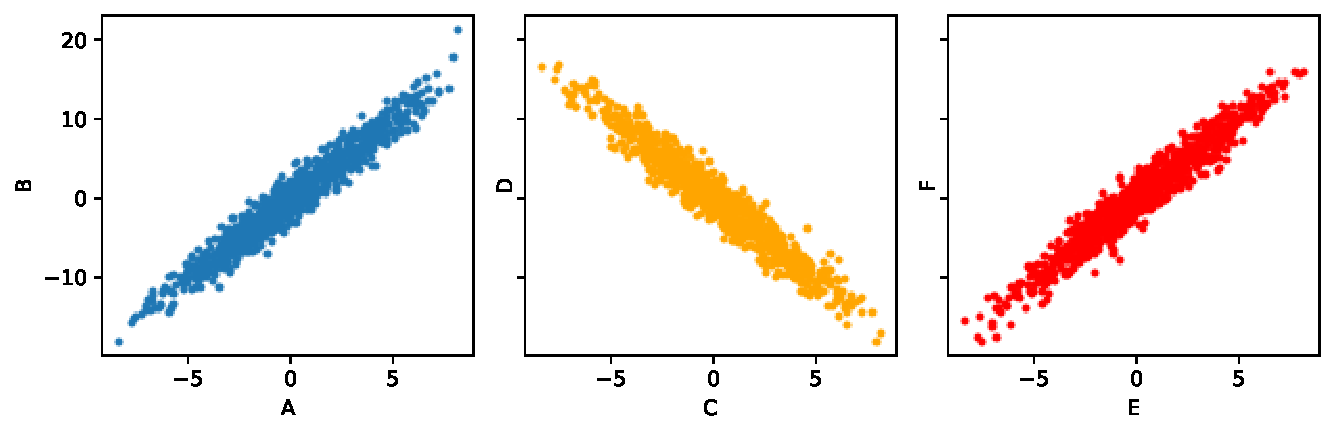
\includegraphics[width=\linewidth]{images/4_gaps/no2ind}
    \caption[Example of a 2D distribution where the pairwise matching is not enough]{
        Example of a 2D distribution where the pairwise matching would not be accurate enough.
        Pairwise tests would tell us that $A$ matches $C$ and $E$; and that $B$ matches $D$ and $F$.
        However, we $A,B$ does not match $C,D$.
    }
    \label{fig:pairwise_ind}
\end{figure}

Therefore, a solution to our research question must take multidimensionality into account.

To bridge this gap, we propose the concept of \glspl{EDD}, which is inspired by the idea of
\glspl{IND} from the relational algebra:

\begin{displayquote}
An inclusion dependency between column A of relation
R and column B of relation S, written $R.A \subseteq S.B$, or $A \subseteq B$
when the relations are clear from the context, asserts that each
value of A appears in B. Similarly, for two sets of columns X
and Y , we write $R.X \subseteq S.Y$ , or $X \subseteq Y$ , when each distinct
combination of values in X appears in Y \cite{abedjan2015}
\end{displayquote}

The definition of \gls{IND} is based on set theory, which is not directly applicable to
numeric data where measures are in the real domain (e.g. spatial coordinates) and usually
have an associated uncertainty that may or may not be explicitly stored.

However, this definition can be naturally reformulated in terms of
equality of distribution $X \eqdist Y: F_X(x) = F_Y(x) \; \forall x$, where $F_X$ and
$F_Y$ are the cumulative distribution functions of X and Y, respectively:

\begin{definition}
An equally-distributed dependency between a set of columns X from
of relation R and a set of columns Y of relation S, written $R.X \eqdist S.Y$ or
$X \eqdist Y$, asserts that the values of X and Y follow the same probability distribution.
\label{def:eqdist}
\end{definition}

The term \emph{arity} refers to the cardinality of the sets of attributes $X$ and $Y$. For instance, if $|X| = 1$, we talk about unary \glspl{EDD}; if $|X| = 2$,
binary or 2-\glspl{EDD}; and, in general, for $|X| = n$, $n$-ary \glspl{EDD}.

Finding high arity \glspl{IND} is a NP-hard problem \cite{kantola1992}.
For instance, for two sets of $n$ attributes in $R$ and $S$,
there are $n!$ different possible permutations to check.
In comparison, finding unary \glspl{IND} seems a relatively simple problem,
as the worst case has complexity $O(n^2)$. Nonetheless,
testing over real files may require expensive input/output operations.
Furthermore, as we will see later, false positives at this stage can quickly make
finding high arity \glspl{IND} unfeasible. This is because the search space tends to grow exponentially
with the number of one-attribute matches, making unary \glspl{IND} search time much less important
than reducing the number of false positives.

We used a published experimental evaluation~\cite{Dursch2019} as a starting point for
assessing how adequate existing solutions are for our problem. The authors carried out a
set of experiments with thirteen \gls{IND} algorithms, of which seven are for unary \glspl{IND},
four for $n$-ary \glspl{IND}, and two for both types. A more recent survey confirms that this
work contains the current state-of-the-art for Inclusion
Dependencies~\cite{kossmann_data_2022}.

We will now describe briefly the $n$-ary finding
algorithms evaluated by the authors and discuss their suitability for our needs.

\subsection{n-INDs finding algorithms}
\label{sec:nind_finding}
\begin{figure}[ht]
    \centering
    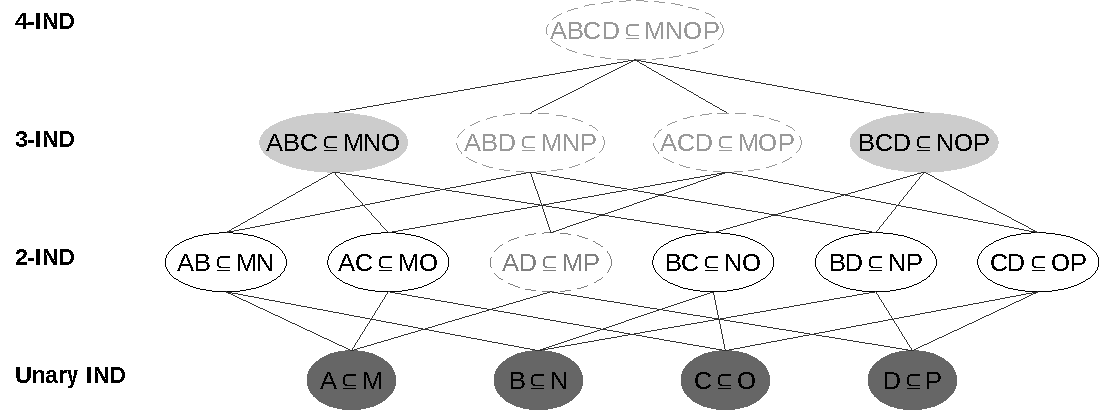
\includegraphics[width=\linewidth]{images/5_presq/lattice}
    \caption[Example structure of the search space as a lattice for an initial set
        of 4 unary \glslongpluralkey {IND}.]{
        Example structure of the search space as a lattice for an initial set
        of 4 unary \glspl{IND}.
        As an illustration, if the 2-INDs surrounded by a solid line were valid,
        a bottom-up traversal would only need checking the validity of the 3-INDs with a 
        gray background since the others could not be valid.
    }
    \label{fig:lattice}
\end{figure}

Given two relations $R$ and $S$, with attributes A and B respectively,
a unary Inclusion Dependency (uIND) exists if $R.A \subseteq S.B$.
More generally, for two sets of attributes $X$ and $Y$, both of cardinality $n$, an
$n$-ary Inclusion Dependency (nIND) exists if every combination of values in X appears in Y
\cite{DeMarchi2002,abedjan2015}.

Given a set $U$ of valid uINDs, the search space for
higher-arity candidates is defined by its power set and a partial order relation
called specialization~\cite{DeMarchi2002}:

\begin{definition}
    \label{def:specialization}
    Let $I_1 = R[X] \subseteq S[Y]$ and
    $I_2 = R'[X'] \subseteq S'[Y']$. $I_1$ \textbf{specializes} $I_2$ (denoted $I_1 \prec I_2)$ iff
    
    \begin{enumerate}
        \item $R = R'$ and $S = S'$.
        \item $X$ and $Y$ are sub-sequences of $X'$ and $Y'$, respectively.
    \end{enumerate}
    
    We can also say that $I_2$ \textbf{generalizes} $I_1$.
\end{definition}

\begin{example}
$(R[AB] \subseteq S[EF]) \prec (R[ABC] \subseteq S[EFG])$. However,
$R[AB] \subseteq S[DE]) \nprec (R[ACD] \subseteq S[DFG])$
\end{example}

This partial order enables us to structure the search space as a lattice, as exemplified in figure
\ref{fig:lattice}. Most solutions leverage this property to explore the search space bottom-up
---from level $k$ to $k$+1--- or top-down ---from level $k$ to $k$--1--- order.

\textsc{Mind}~\cite{DeMarchi2002} is a bottom-up approach: it starts
from a set of known, satisfied unary \glspl{IND} and builds higher arity candidates
combining them.
These new candidates are then validated against the database, and those satisfied
are used for computing the next-level candidates until no more candidates are available.

\Zigzag~\cite{DeMarchi2003zigzag} starts with a \textsc{Mind} bottom-up approach
up to a given arity $n \ge 2$. Then, it uses all satisfied \glspl{IND} to initialize a \textit{positive border}
and the non-satisfied to initialize a \textit{negative border}. The set of satisfied \glspl{IND}
is used to generate the set of candidates with the highest arity possible, called
\textit{optimistic border},
which is then validated against the database. This is the bottom-up part of the search.
Valid candidates are directly added to the positive border.
Invalid candidates are treated depending on how many tuples are different between relations.
Those above a given threshold (too many different tuples) are added to the negative border.
Those below are top-down traversed, from level $n$ to $n$--1, validated, and then added
to the positive border if they are satisfied. The algorithm then iterates, building a new
optimistic border until it is impossible to generate new \glspl{IND}. The optimistic approach
can prune the search space very aggressively when there are high-arity \glspl{IND},
but when most arities are low,  \textsc{Mind} may perform better.

\Find~\cite{koeller2003discovery} is based on the equivalence
between finding $n$-INDs and finding cliques on $n$-uniform hypergraphs (a generalization
of the concept of a graph where each edge connects $n$ nodes). Each unary \gls{IND} corresponds
to a node, and an $n$-IND corresponds to an edge on an $n$-uniform hypergraph.
Once such a graph is built, each \gls{IND} corresponds to a clique and maximal \glspl{IND}
correspond to maximal cliques. They present the \Hyperclique algorithm,
capable of finding maximal cliques performantly, which can be mapped back to candidate
maximal \glspl{IND}. These are finally validated using database queries.
As \Zigzag, \Find starts with a bottom-up
approach to look for maximal cliques (i.e., potential maximal \glspl{IND}). The invalid ones
are used to generate a new ($n$+1) uniform graph. This is a stage that corresponds to the top-down
traversal.

While these three algorithms were evaluated on \glspl{IND} between relational datasets
and with attributes that can be directly compared (i.e. from discrete domains), their
traversal of the search space and their validation steps are well decoupled. They
can be easily be adapted to the equality-of-distribution statistical tests.

Furthermore, the reference benchmark shows that \Mind, \Find
and \Zigzag have a comparable run-time, sometimes even
faster than the alternatives.
While \textsc{Faida} is generally faster, its
validation strategy requires computing hashes over the
attributes and their combinations, which is inapplicable
for continuous data that can very possibly have an associated uncertainty.

From the three suitable candidates, \Mind's bottom-up approach can be performant enough for
relatively low arity \gls{IND} relations. However, it has one substantial disadvantage:
it requires an exponential number of tests, prohibitive for higher arity \glspl{IND}.
Both \Zigzag and \Find overcome this limitation by alternating between \emph{optimistic}
(top-down) and \emph{pessimistic} (bottom-up) traversals.
Finally, \Find maps the search of \glspl{IND} to the search of maximal cliques. We know that
using statistical tests will introduce unavoidable false negatives, which would
translate into missing edges.
A clique with missing edges is a quasi-clique, and finding quasi-cliques, while at least
as hard as finding cliques, is doable.

\subsection{Foreign Key Discovery}

We briefly survey this area since we consider it complementary to
\gls{IND} discovery. A \gls{FK} constrain on an attribute
$A$ over a \gls{PK} $B$ implies that all values present on $A$ must also be
present on $B$.
Therefore, there exists an inclusion dependency between $A$ and $B$.
However, the reverse is not necessarily true. For instance, two auto-increment attributes from
two different relations may have an accidental \gls{IND} with no semantic meaning.

To distinguish between accidental and meaningful \glspl{IND}, Rostin \etal~\cite{Rostin2009} propose to
train machine learning models over a set of features extracted from positive
\gls{PK}/\gls{FK} relations and negative, non-meaningful \glspl{IND}. However, their proposal
is limited to unary \glspl{IND}.

Zhang \etal~\cite{Zhang2010} present an algorithm capable of handling multi-column
\gls{PK}/\gls{FK} relations.
They define the concept of \emph{Randomness Test}, which assumes that an \gls{FK} is a representative
sample of a \gls{PK} and, therefore, should follow a similar distribution.
They use an approximation of the \gls{EMD} ---the cost of transforming one distribution into another---
to measure the similarity between \gls{PK} and \gls{FK}.
Their algorithm ranks \gls{PK}/\gls{FK} candidates by distance ---closest first--- and selects
the top $X\%$, where $X$ must be chosen to balance precision and recall.

More recently, Jian \etal~\cite{jiang_holistic_2020} introduced an approach that identifies
both \gls{PK} and \gls{FK} holistically. They validate Zhang's concept of \emph{Randomness}
and propose a simplified estimator that treats each attribute separately. They do not need
the \glspl{PK} to be known but require a list of \glspl{IND} as input.

It is worth noting that even though the latter two publications use the idea of the
\gls{FK} being a random sample of the \gls{PK}, their methods use the \emph{distance} between
distributions for ranking candidates~\cite{Zhang2010} or as a feature~\cite{jiang_holistic_2020}.
Our method is based, however, on statistical hypothesis testing\footnotemark.

\footnotetext{While the \gls{EMD} could be used as a test statistic, it would be computationally
expensive~\cite{hallin2021multivariate}.}

\subsection{Complementarity}

\textsc{ReDiscover}~\cite{alawini2016} uses machine learning techniques, such as
\glspl{SVM}, to identify matching columns between scientific tabular data.
The author defines different ways in which datasets may be related:
containment, partial containment, augmentation, completion, equality, \ldots
This solution focus does not only focus on correspondences (i.e., $A$ is a subset of $B$),
but it also pays attention to the semantics of the \emph{relationship} (i.e., $A$
is a selection of $B$).
Yet, this system focuses mainly on the correspondence between \emph{individual columns},
which is insufficient for spatial and coincidence associations, as they are multidimensional.
We are left only with a set of pairwise correspondences that may not be enough to cross-match
tuples between files.

\subsection{Schema Homogenization}

For completeness, table~\ref{tab:missing_middleware} classifies these solutions,
expanding on the result from the literature mapping shown in chapter~\ref{chapter:literature_review}.

\begin{table}[ht]
    \centering
    \begin{tabularx}{\linewidth}{p{7em} >{\raggedright}X >{\raggedright}X X}
    \hline
    \multicolumn{4}{l}{\textbf{Middleware}} \\
    \hline
    \textit{Schema \mbox{Homogenization}} &
    \gls{IND}     \cite{DeMarchi2002,DeMarchi2003zigzag,koeller2002integration} &
    \gls{FK}      \cite{Rostin2009,Zhang2010,jiang_holistic_2020} &
    Complementarity \cite{alawini2016} \\
    \hline
    \end{tabularx}
    \caption[Articles under Schema Homogenization]{
    Expansion of Idreos~\cite{Idreos2015} classification with \emph{Schema Homogenization}}
    \label{tab:missing_middleware}
\end{table}


\section{Proposed solution}
In the following chapter, we propose a novel algorithm, \PresQ, that
can recover multidimensional correspondences between datasets with different,
undocumented --- or unknown --- schemas. \PresQ relies on statistical tests to
accept or discard these correspondences.

To complement this method, chapter~\ref{chapter:som} describes a multidimensional
statistical test based on \gls{SOM} offering additional interpretability. It can be
used with \PresQ for studying with more details accepted or rejected correspondences,
or afterward over the merged dataset for clustering or as a pre-processing for nearest-neighbor
coincidence search~\cite{silva2011som}.

Appendix~\ref{appendix:prototypes} briefly describes the preliminary ideas that were
discarded during the phase of \emph{Embodiment Design}.
